\section{Produktübersicht}
\subsection{Systemarchitektur}

\begin{figure} [h]	
	\centering
	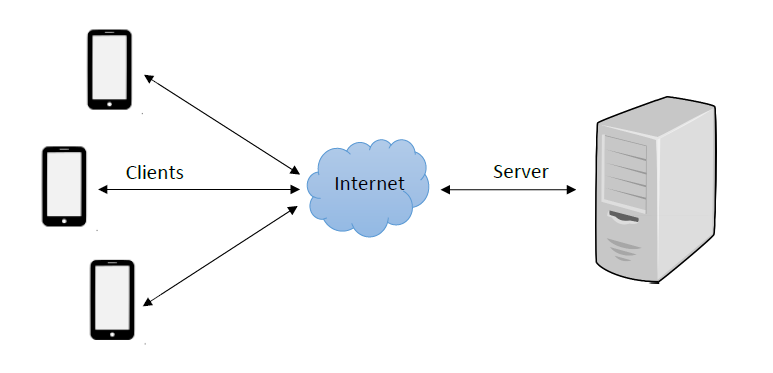
\includegraphics[scale = 0.8]{res/clientServerArchitektur.png}
\end{figure}
Die Client-Server-Architektur wird verwendet, da mehrere Mobiltelefone nebeneinander ohne konkrete Kenntnis voneinander zu haben, Ressourcen des Servers anfragen. Dieser wertet die Anfrage aus und liefert eine Antwort zurück an den Client. \\
In unserem Fall steht jeder Benutzer über einen zentralen Server in Verbindung mit seinen Gruppen und kann so z.B. die Standorte der anderen Mitglieder anfragen und bekommt diese dann vom Server geliefert.

\subsection{Szenarien}
\subsection{Anwendungsfälle}
\subsubsection{Musskriterien}
\subsubsection{Wunschkriterien}